%%%%%%%%%%%%%%%%%%%%%%%%%%%%%%%%%%%%%%%%%%%%%%%%%%%%%%%%%%%%%%%%%%%%%%%%%%%%%%%%%
%%%  LaTeX document class of the thesis of the Gyeonggi Science High School   %%%
%%%  Last edition 2015.11.13 by Chinook Mok                                   %%%
%%%  Continously being modified by gshslatexintro after 2016.02.02.           %%%
%%%  Check the latest version at : latex.gs.hs.kr                             %%%
%%%  Also refer to https://www.facebook.com/gshstexsociety                    %%%
%%%%%%%%%%%%%%%%%%%%%%%%%%%%%%%%%%%%%%%%%%%%%%%%%%%%%%%%%%%%%%%%%%%%%%%%%%%%%%%%%

\documentclass[twoside,11pt]{gshs_thesis}
\RequirePackage[nonfrench]{kotex}
% 이곳에 필요한 별도의 패키지들을 적어넣으시오.
%\usepackage{...}
\usepackage{verbatim} % for commment, verbatim environment
\usepackage{spverbatim} % automatic linebreak verbatim environment
\usepackage{amsmath}
\usepackage{amssymb}
\usepackage{kotex}
\usepackage{tabu}
\usepackage{booktabs}
\usepackage{siunitx}
\usepackage{graphicx}
\usepackage{subfig}
\usepackage{multirow,makecell}
\usepackage{listings}
\lstset{
	basicstyle=\small\ttfamily,
	columns=flexible,
	breaklines=true
}

% -----------------------------------------------------------------------
%                   이 부분은 수정하지 마시오.
% -----------------------------------------------------------------------
\titleheader{졸업논문청구논문}
\school{과학영재학교 경기과학고등학교}
\approval{위 논문은 과학영재학교 경기과학고등학교 졸업논문으로\\
졸업논문심사위원회에서 심사 통과하였음.}
\chairperson{박용선}
\examiner{강동일}
\apprvsign{(인)}
\korabstract{초 록}
\koracknowledgement{감사의 글}
\korresearches{연 구 활 동}

%: ----------------------------------------------------------------------
%:                  논문 제목과 저자 이름을 입력하시오
% ----------------------------------------------------------------------
\title{Orion A Cloud의 쌍극 방출류의 성질} %한글 제목
\engtitle{Properties of bipolar outflows of the Orion A Cloud} %영문 제목
\korname{이 선 재} %저자 이름을 한글로 입력하시오 (글자 사이 띄어쓰기)
\engname{Lee, Seon Jae} %저자 이름을 영어로 입력하시오 (family name, personal name)
\chnname{李 善 在} %저자 이름을 한자로 입력하시오 (글자 사이 띄어쓰기)
\studid{16072} %학번을 입력하시오

%------------------------------------------------------------------------
%                  심사위원과 논문 승인 날짜를 입력하시오
%------------------------------------------------------------------------
\advisor{Park, Kiehyun}  %지도교사 영문 이름 (family name, personal name)
\judgeone{} %심사위원장
\judgetwo{}   %심사위원1
\judgethree{박 기 현} %심사위원2(지도교사)
\degreeyear{2019}   %졸업 년도
%\degreedate{2015}{11}{13} %논문 승인 날짜 양식
\degreedate{2018. 7. 21} %논문 승인 날짜 양식1
\degreedatekor{2018년 7월 21일} %논문 승인 날짜 양식2

%------------------------------------------------------------------------
%                  논문제출 전 체크리스트를 확인하시오
%------------------------------------------------------------------------
\checklisttitle{[논문제출 전 체크리스트]} %수정하지 마시오
\checklistI{1. 이 논문은 내가 직접 연구하고 작성한 것이다.} %수정하지 마시오
% 이 항목이 사실이라면 다음 줄 앞에 "%"기호 삽입, 다다음 줄 앞의 "%"기호 제거하시오
%\checklistmarkI{$\square$}
\checklistmarkI{$\text{\rlap{$\checkmark$}}\square$}
\checklistII{2. 인용한 모든 자료(책, 논문, 인터넷자료 등)의 인용표시를 바르게 하였다.} %수정하지 마시오
% 이 항목이 사실이라면 다음 줄 앞에 "%"기호 삽입, 다다음 줄 앞의 "%"기호 제거하시오
%\checklistmarkII{$\square$}
\checklistmarkII{$\text{\rlap{$\checkmark$}}\square$}
\checklistIII{3. 인용한 자료의 표현이나 내용을 왜곡하지 않았다.} %수정하지마시오
% 이 항목이 사실이라면 다음 줄 앞에 "%"기호 삽입, 다다음 줄 앞의 "%"기호 제거하시오
%\checklistmarkIII{$\square$}
\checklistmarkIII{$\text{\rlap{$\checkmark$}}\square$}
\checklistIV{4. 정확한 출처제시 없이 다른 사람의 글이나 아이디어를 가져오지 않았다.} %수정하지 마시오
% 이 항목이 사실이라면 다음 줄 앞에 "%"기호 삽입, 다다음 줄 앞의 "%"기호 제거하시오
%\checklistmarkIV{$\square$}
\checklistmarkIV{$\text{\rlap{$\checkmark$}}\square$}
\checklistV{5. 논문 작성 중 도표나 데이터를 조작(위조 혹은 변조)하지 않았다.} %수정하지 마시오
% 이 항목이 사실이라면 다음 줄 앞에 "%"기호 삽입, 다다음 줄 앞의 "%"기호 제거하시오
%\checklistmarkV{$\square$}
\checklistmarkV{$\text{\rlap{$\checkmark$}}\square$}
\checklistVI{6. 다른 친구와 같은 내용의 논문을 제출하지 않았다.} %수정하지 마시오
% 이 항목이 사실이라면 다음 줄 앞에 "%"기호 삽입, 다다음 줄 앞의 "%"기호 제거하시오
%\checklistmarkVI{$\square$}
\checklistmarkVI{$\text{\rlap{$\checkmark$}}\square$}

\usepackage{tocloft}
\setlength{\cftbeforesecskip}{0pt}
\setlength{\cftbeforesubsecskip}{0pt}
\setlength{\cftbeforesubsubsecskip}{0pt}
\begin{document}
%\renewcommand\baselinestretch{1.2} % line spacing in the paragraph
%\baselineskip=22pt plus1pt         % line spacing in the paragraph
\baselineskip=2.2em         % line spacing in the paragraph

\maketitle  % command to print the title page with above variables
\setcounter{page}{1}
%---------------------------------------------------------------------
%                  영문 초록을 입력하시오
%---------------------------------------------------------------------
\begin{abstracts}     %this creates the heading for the abstract page
	\addcontentsline{toc}{section}{Abstract}  %%% TOC에 표시
	\noindent{
Stars are born when matter from interstellar molecular clouds fall to its center to increase the mass of the protostar. Bipolar outflows are formed to remove the excess angular momentum of falling matter. Intensities of outflows are known as to be in a close relationship with their bolometric luminosity and evolutionary stages. In this paper, data from Institute for Radio Astronomy in the Millimeter Range (IRAM) 30$\,$m Telescope and Taeduk Radio Astronomy Observatory (TRAO) are used. IRAM was used to map $^{12}\textrm{CO}$ J = 2 - 1 over Orion A molecular cloud. TRAO was used to map $^{13}\textrm{CO}$ J = 1 - 0 over the same region. Outflows were observed and measured by drawing contour maps and line profiles of  red/blue shifted components. Outflows could be detected better if the energy level of the emission line is higher. Also, the correlation between a protostar's luminosity and outflow force have been confirmed.
	} 
\end{abstracts}

\begin{abstractskor}
	별은 성간분자운의 물질이 중심으로 떨어져 원시성의 질량을 증가시켜야만 탄생된다. 이 과정에서 중심으로 떨어지는 물질의 각운동량을 제거하기 위해 방출류가 발생한다. 여기서 방출류의 세기는 원시성의 진화 단계와 광도와 관련이 있다고 알려져 있다. 이를 새로 관측된 데이터를 사용하여 보다 좋은 방출류 측정 방법과 기존의 연구를 검증해 보려고 한다.이 연구에서는  Institute for Radio Astronomy in the Millimeter Range 30$\,$m (IRAM) 망원경으로 관측한 $^{12}$CO J = 2 - 1 관측 자료와 대덕 전파 망원경(Taeduk Radio Astronomy Observatory, TRAO)으로 관측한 $^{13}$CO J = 1 - 0 천이 선 자료를 이용하였다. 두 자료 모두 Orion A Cloud 영역을 담고 있다. 빠른 속도 성분을 가진 적색/청색편이된 성분의 contour map을 그려 방출류를 관찰하고 방출류의 세기를 구하였다. 방출류의 세기와 원시성의 광도가 대체적으로 비례한다는 것을 알 수 있었다. 그리고 천이 선의 에너지 준위가 높을수록 방출류를 더 잘 검출할 수 있음을 확인할 수 있었다.
\end{abstractskor}
%----------------------------------------------
%   Table of Contents (자동 작성됨)
%----------------------------------------------
\cleardoublepage
\addcontentsline{toc}{section}{Contents}
\setcounter{secnumdepth}{3} % organisational level that receives a numbers
\setcounter{tocdepth}{3}    % print table of contents for level 3
\baselineskip=2.2em
\tableofcontents


%----------------------------------------------
%     List of Figures/Tables (자동 작성됨)
%----------------------------------------------
\cleardoublepage
\clearpage
\listoffigures	% 그림 목록과 캡션을 출력한다. 만약 논문에 그림이 없다면 이 줄의 맨 앞에 %기호를 넣어서 코멘트 처리한다.

\cleardoublepage
\clearpage
\listoftables  % 표 목록과 캡션을 출력한다. 만약 논문에 표가 없다면 이 줄의 맨 앞에 %기호를 넣어서 코멘트 처리한다.


%%%%%%%%%%%%%%%%%%%%%%%%%%%%%%%%%%%%%%%%%%%%%%%%%%%%%%%%%%%
%%%% Main Document %%%%%%%%%%%%%%%%%%%%%%%%%%%%%%%%%%%%%%%%
%%%%%%%%%%%%%%%%%%%%%%%%%%%%%%%%%%%%%%%%%%%%%%%%%%%%%%%%%%%
\cleardoublepage
\clearpage
\renewcommand{\thepage}{\arabic{page}}


%-----------------------------------------------------
%  Introduction
%-----------------------------------------------------

\section{Introduction}

Stars are formed in molecular clouds by gravitational accretion. In the early stages of star formation, young stellar objects(YSOs) are still embedded in the molecular clouds, increasing its mass and temperature by accretion of interstellar medium around it. Since the angular momentum is conserved while matter is accreted, matter near the surface of the protostar spins quickly, which stops more accretion. Since angular momentum is removed by jets called bipolar outflows, outflows are observed with size proportional to the mass accreted to the protostar\cite{Bontemps}. 
It is already known that the accretion rate and the luminosity correlates to each other \cite{Kang}. The outflow force decreases as protostars evolve from Class 0 to Class I, which means the strength that the protostar pulls interstellar matter decreases as time passes.             
In this study, I will observe the protostars and their outflows of Orion A Cloud. First, I will select the protostars that outflows can be detected from the Spitzer and the Herchel catalogues \cite{Spitzer, HerschelFurlan}. By using different data sets observed by different observatries and different wavelengths, I will identify the outflows. I will recheck the correlation between the outflow force and its bolometric luminosity. Also, I will compare outflow forces calculated using different wavelengths of light. 

\newpage
\section{Obervations and Data Reduction}

\subsection{Observation Region}
The Orion region consists of two giant molecular clouds, the Orion A and B clouds. This research covers the Orion A Cloud. The Orion A Cloud covers about $29 \textrm{deg}^2$ of the sky and its distance is about 450$\,$pc \cite{Oriondistance}. The total mass is estimated to be about $10^5 M_{\odot}$. It contains several hot molecular cores, such as the BN-KL nebula. It is known that the Orion Cloud was formed by a collision and fragmentation between two giant molecular clouds about 60 million years ago. The effects of the collision can be seen nowdays. There is a big velocity gradient along the declination axis. On the north side of the Orion A Cloud (OMC 2) shows about 12$\,$km/s but on the south end (L1641) it has velocity about 5$\,$km/s \cite{Schulz}.

\subsection{Observation Data}
The $^{12}$CO(J = 2 - 1, $230.538\,$GHz) data was observed with the IRAM 30$\,$m telescope in Granada, Spain, in 2013. The spatial beamwidth was 11", and the spectral resolution was 0.4$\,$km/s. The noise level was 0.2$\,$K. It only covers the north region of the Orion A cloud \cite{Berne}. \\
The $^{12}$CO(J = 1 - 0, $115.271\,$GHz) data was observed with the NRO 45m telescope in Nobeyama, Japan.  \\
The $^{13}$CO(J = 1 - 0, $110.201\,$GHz) and the $\textrm{C}^{18}\textrm{O}$(J = 1 - 0, 109.782GHz) was observed at Taeduk Radio Astronomy Observatory (TRAO) 13.7$\,$m telescope in 2017. The spatial beamwidth was 45", and the spectral resolution was 0.05$\,$km/s. The noise level was 0.4$\,$K.\\
$^{13}$CO and $\textrm{C}^{18}\textrm{O}$ lines are optically thin lines which can trace most of the matter on the line of sight, contrasting to $^{12}$CO lines which are so optically oblique that it can only trace the outermost part of the molecular core. In this study, I used TRAO data to determine the protostar's velocity and linewidth which are the kinematic properties of the envelope. Then, I will trace the outflow jets using $^{12}$CO data.
\begin{figure}[h]
	\begin{center}
		\begin{tabular}{cc}
			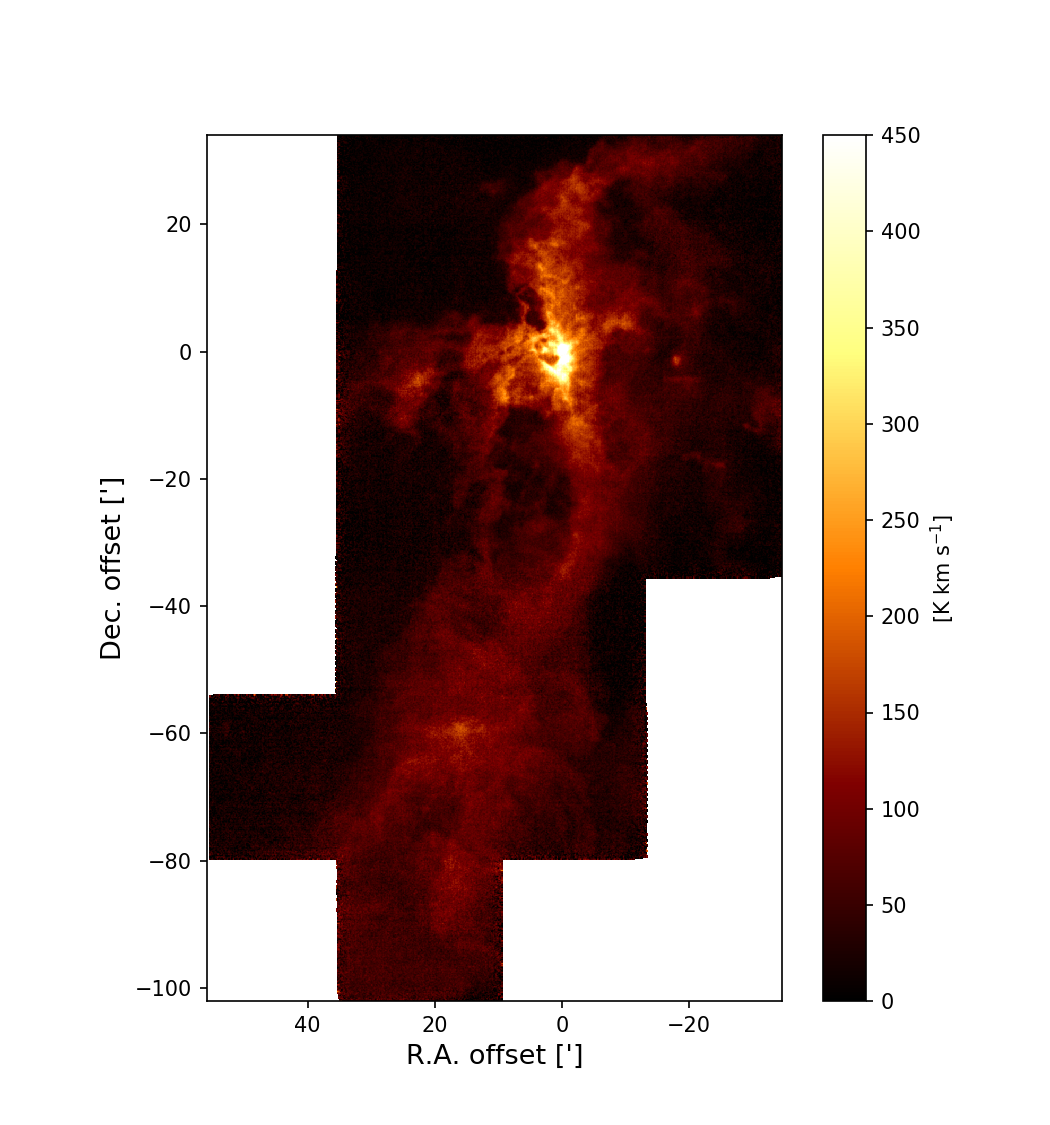
\includegraphics[width=0.4\textwidth]{RNE_12CO_Orion.png} & 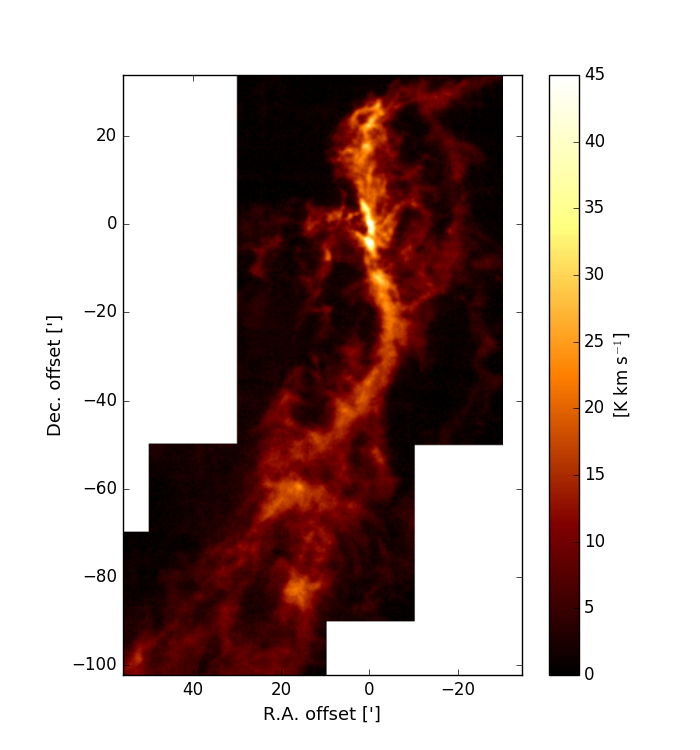
\includegraphics[width=0.4\textwidth]{Orion_13CO_intmap.png}
		\end{tabular}
	\end{center}
	\caption{Orion A $^{12}$CO (J = 2 - 1) intergrated intensity map(left) $^{13}$CO intergrated intensity map(right).}
\end{figure}

\subsection{Identification of Outflows}
Data obtained by observing with radio waves are summed over the line of sight, which tells us the distribution of matter which has relative radial velocity to the observer. The envelope around the protostar is static or is contracting slowly to the protostar itself, but outflow jets have big velocity components from each pole. If the inclination of the outflows are not zero, it would be seen as jets are moving closer or further from the observer. In this study, $^{13}$CO and $\textrm{C}^{18}\textrm{O}$ lines were used to get the velocity distribution of the protostar. By using Gaussian fitting, I calculated the protostar’s central velocity($v_{cen}$) and the full width at half maximum(FWHM). The intervals of the red/blue lobes were defined by how far is it from the center velocity and how strong the intensity is. \\
Because the emission lines of $^{12}$CO are optically thicker than other lines, it is appropriate to trace the outflows with $^{12}$CO lines. I drew contour maps to find out if bipolar outflows existed with the protostar at its center. To check if the red blue lobes that are found are outflows from the same protostar I checked the $^{12}$CO, $^{13}$CO, $\textrm{C}^{18}\textrm{O}$ lines from the red peak, blue peak, and the center points. For each outflows confirmed, I calculated the column density and the momentum force. \\

\newpage

\section{Results}

\begin{table}[h!]
	\begin{center}
		\begin{tabular}{c|c|c|c|c}
			\toprule
			& \multicolumn{2}{c|}{coordinates} & $\mathbf{L_{bol}}$ & $\mathbf{T_{bol}}$\\
			\textbf{Name} & \textbf{RA} & \textbf{Dec} & $\mathbf{L_{\odot}}$ & $\mathbf{K}$\\
			\midrule
			\multicolumn{5}{c}{Orion A Cloud}\\
			\midrule
			\centering
			FIR2 & 05:35:24.3 & -05:08:33.3 & 5.68 & 100.6\\
			FIR3 & 05:35:27.5 & -05:09:32.5 & 360.86 & 71.5\\
			FIR6b & 05:35:23.4 & -05:12:03.2 & 21.93 & 54.1\\
			MMS2 & 05:35:18.3 & -05:00:34.8 & 20.11 & 186.3\\
			MMS5 & 05:35:22.4 & -05:01:14.1 & 15.81 & 42.4\\
			MMS9 & 05:35:26.0 & -05:05:42.4 & 8.91 & 38.1\\
			\midrule
		\end{tabular}
	\end{center}
	\caption{Protostars with observed outflows}
\end{table}

\subsection{Outflow Identification}

The column density can be calculated as the following expression:
\begin{align}
N_{H_2} =& \frac{8\pi \nu^3}{c^3} \frac{1}{(2J_l +3)A}  \notag \\
& \times \frac{Z(T_{ex})}{exp(-E_l / kT_{ex})[1-exp(h\nu / kT_{ex})]} \notag \\
& \times \frac{\int T_B dV}{J(T_{ex})-J(T_{bg})}
\end{align}

\begin{equation}
	J(T) = \frac{h \nu / k}{exp(h\nu / kT)-1}
\end{equation}

In the above equation, $\nu$ is the corresponding frequency of emission line, $c$ is the speed of light, $J_l$ is the rotational quantum number of the lower energy level, $A$ is the Einstein A coefficient, $Z$ is the partition function, $E_l$ is the rotational energy of the lower energy level, $k$ is the Boltzmann's constant, $T_{ex}$ is the excitation temperature of the transitions, $\int T_B dV$ is the integrated intensity measured, $T_{bg}$ is the background radiation temperature. I assumed a local thermal equilibrium(LTE) excitation at an outflow temperature of 50$\,$K \cite{Takahashi}.\\

The mass within one beam can be calculated as the following:

\begin{equation}
M_B =  \frac{\pi}{4} D^2 \theta_B ^2 X[\textrm{CO}] N_{H_2} m_{H_2}
\end{equation}

$D$ is the distance to the objects, $\theta_B$ is the beam size, $m_{H_2}$ is the mass of one hydrogen molecule. $X[\textrm{CO}]$ is the abundance ratio of CO to $\textrm{H}_2$. In this paper, $D = 450\,pc$ and $X[\textrm{CO}] = 10^{-4}$ was used \cite{Hatchell2}.\\



\subsubsection{$^{12}$CO J = 2 - 1 Observations}

\begin{figure}[h!]
	\begin{center}
		\begin{tabular}{cc}
			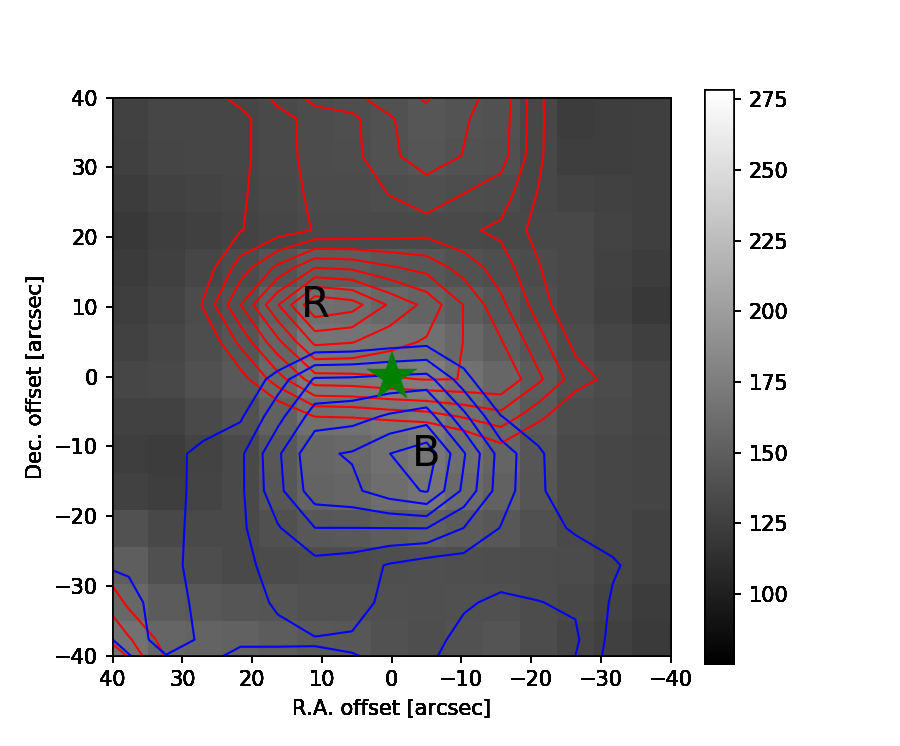
\includegraphics[width=5cm]{Orion_12CO2-1_FIR2_rbcontour_400_modified.png} &   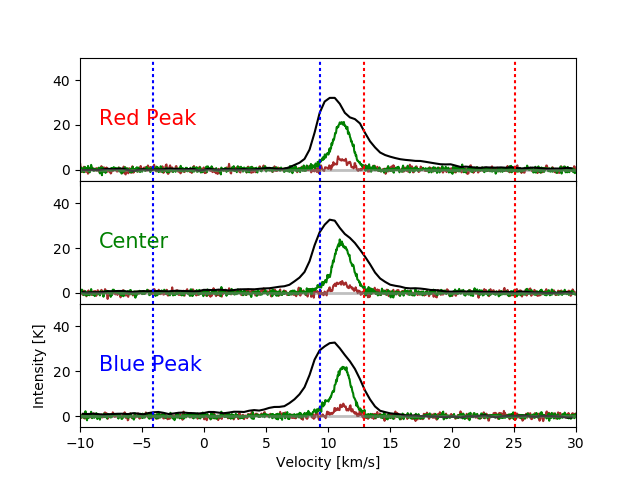
\includegraphics[width=5cm]{Orion_12CO2-1_FIR2_line_profile_400.png} \\
		\end{tabular}
		\label{FIR221}
		\caption{The contour map(left) and the line profile(right) of FIR2. }
	\end{center}
\end{figure}

\begin{figure}[h!]
	\begin{center}
		\begin{tabular}{cc}
			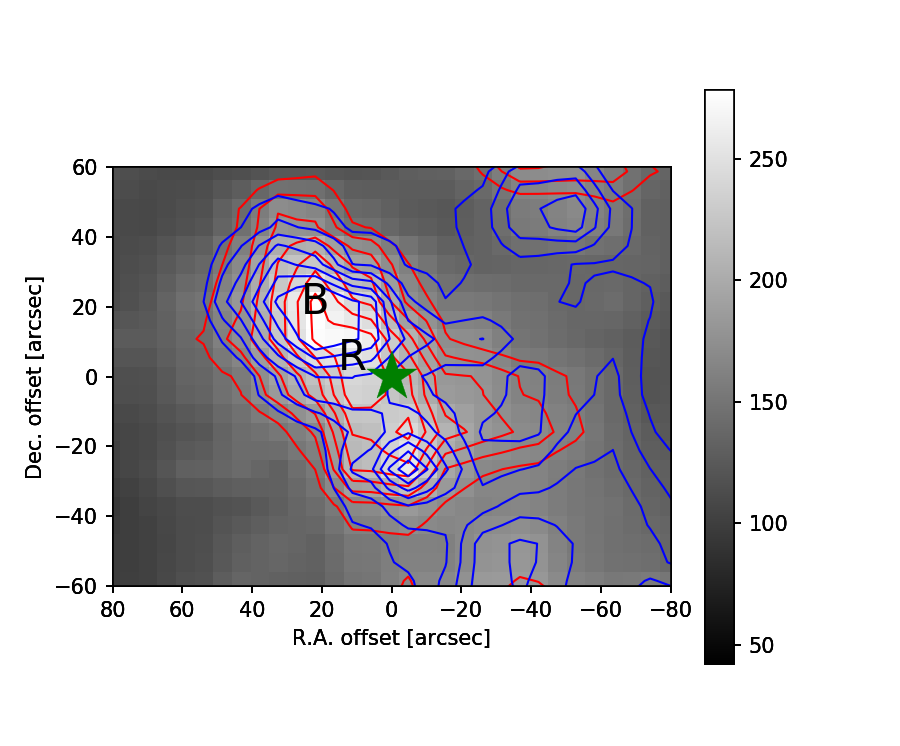
\includegraphics[width=5cm]{Orion_12CO2-1_FIR3_rbcontour_400_modified.png} &   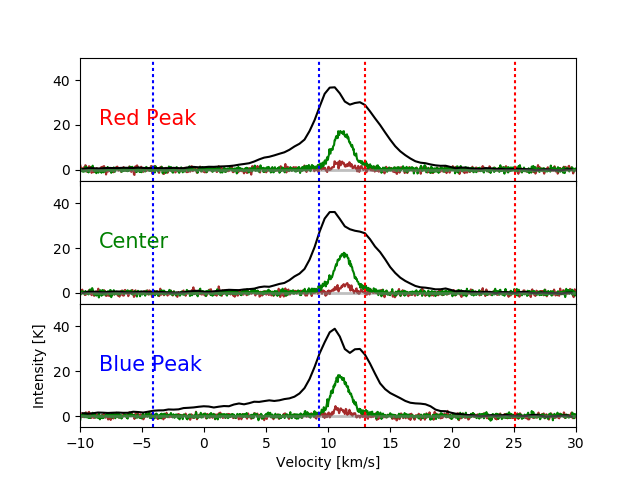
\includegraphics[width=5cm]{Orion_12CO2-1_FIR3_line_profile_400.png}\\
		\end{tabular}
		\label{FIR321}
		\caption{The contour map and the line profile of FIR3. }
	\end{center}
\end{figure}

\begin{figure}[h!]
	\begin{center}
		\begin{tabular}{cc}
			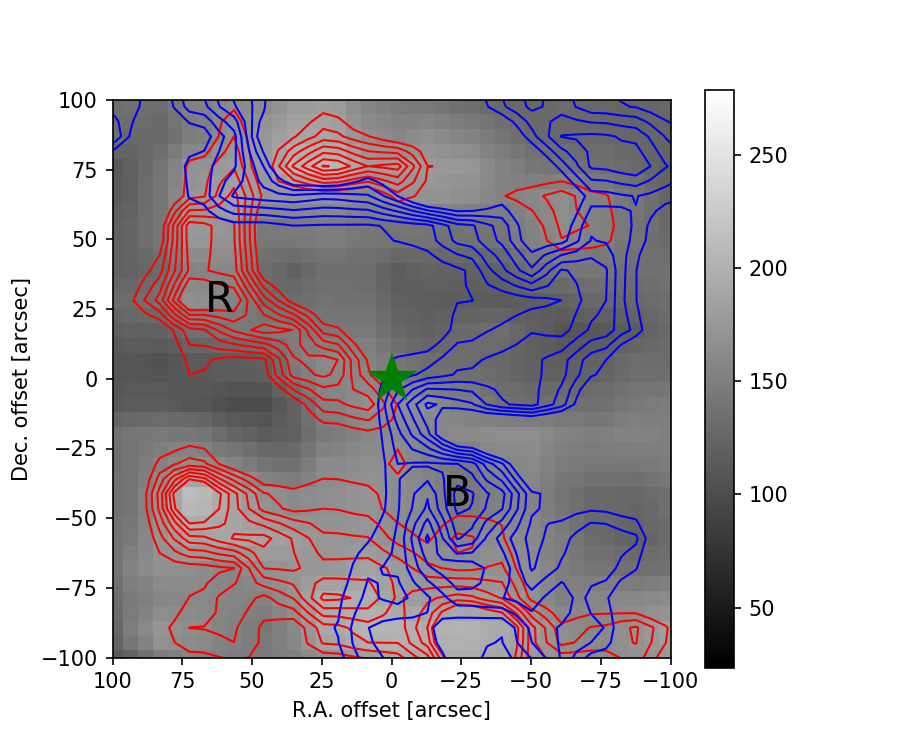
\includegraphics[width=5cm]{Orion_12CO2-1_FIR6b_rbcontour_400_modified.png} &   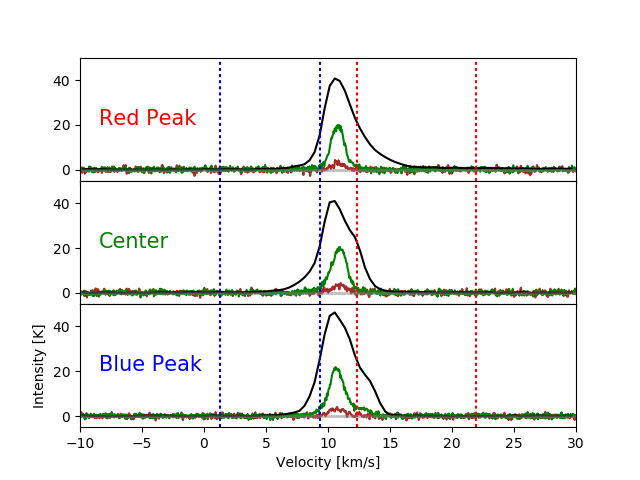
\includegraphics[width=5cm]{Orion_12CO2-1_FIR6b_line_profile_400.png}\\
		\end{tabular}
		\label{FIR6b21}
		\caption{The contour map and the line profile of FIR6b. }
	\end{center}
\end{figure}

\begin{figure}[h!]
	\begin{center}
		\begin{tabular}{cc}
			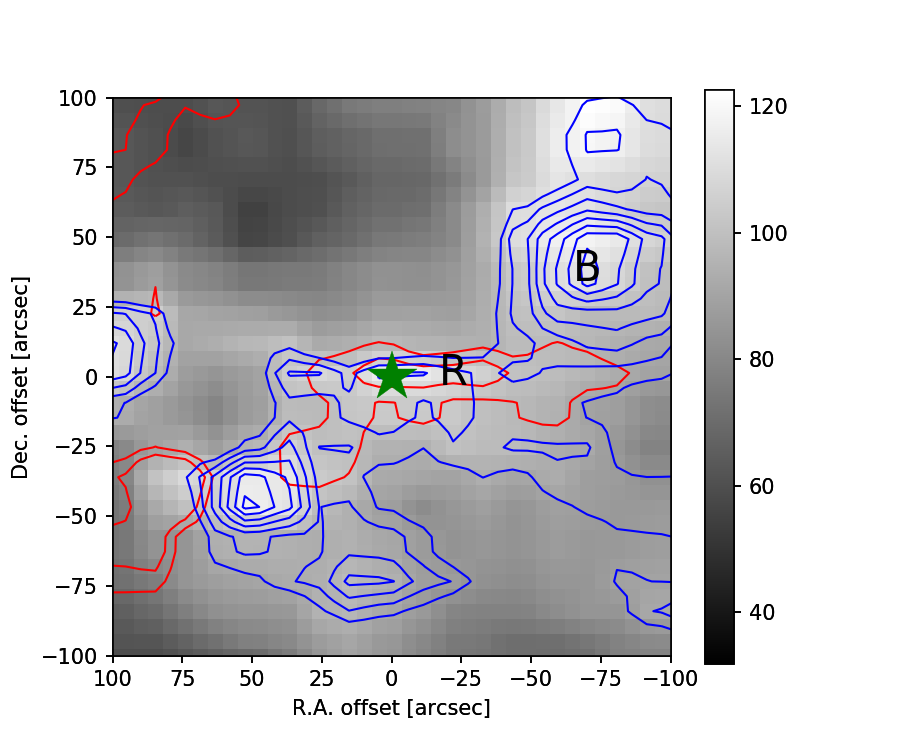
\includegraphics[width=5cm]{Orion_12CO2-1_MMS2_rbcontour_400_modified.png} &   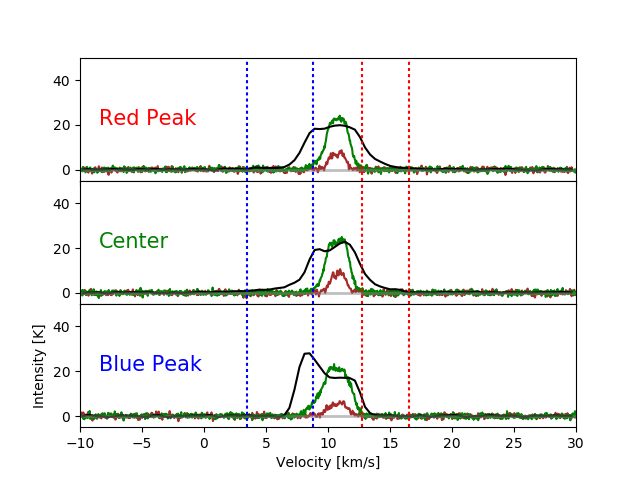
\includegraphics[width=5cm]{Orion_12CO2-1_MMS2_line_profile_400.png} \\
		\end{tabular}
		\label{MMS221}
		\caption{The contour map and the line profile of MMS2. }
	\end{center}
\end{figure}

\begin{figure}[h!]
	\begin{center}
		\begin{tabular}{cc}
			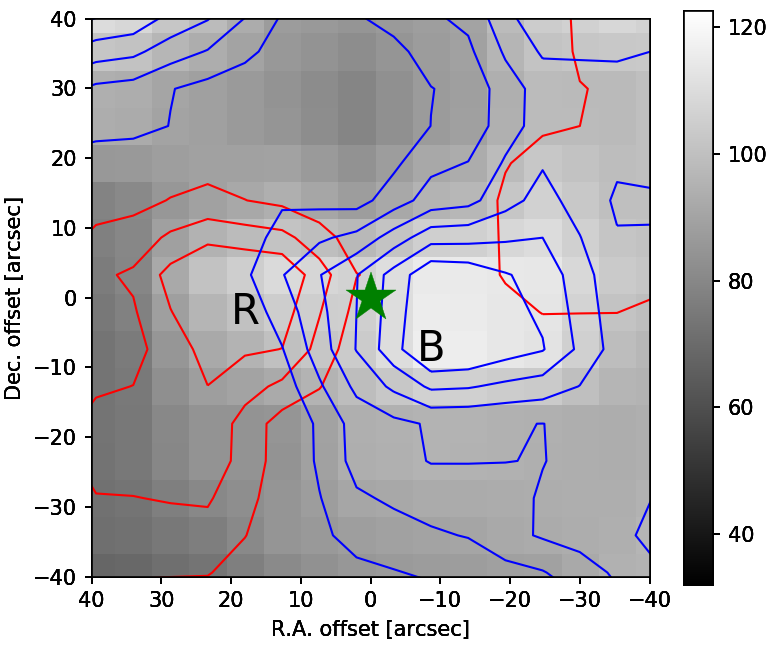
\includegraphics[width=5cm]{Orion_12CO2-1_MMS5_rbcontour_400_modified.png} &   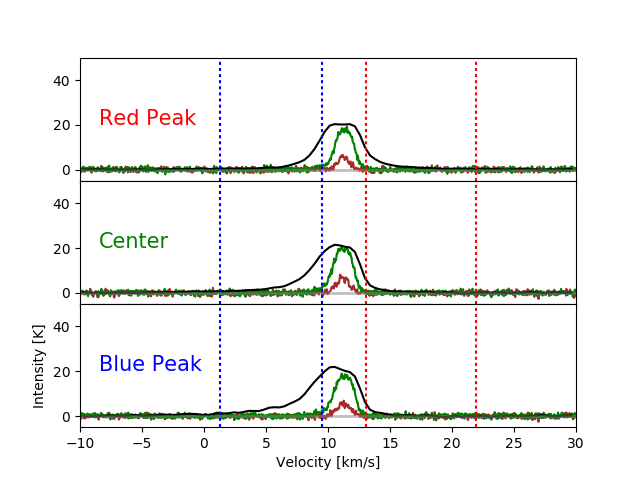
\includegraphics[width=5cm]{Orion_12CO2-1_MMS5_line_profile_400.png} \\
		\end{tabular}
		\label{MMS521}
		\caption{The contour map and the line profile of MMS5. }
	\end{center}
\end{figure}
\clearpage
\newpage
\begin{figure}[h!]
	\begin{center}
		\begin{tabular}{cc}
			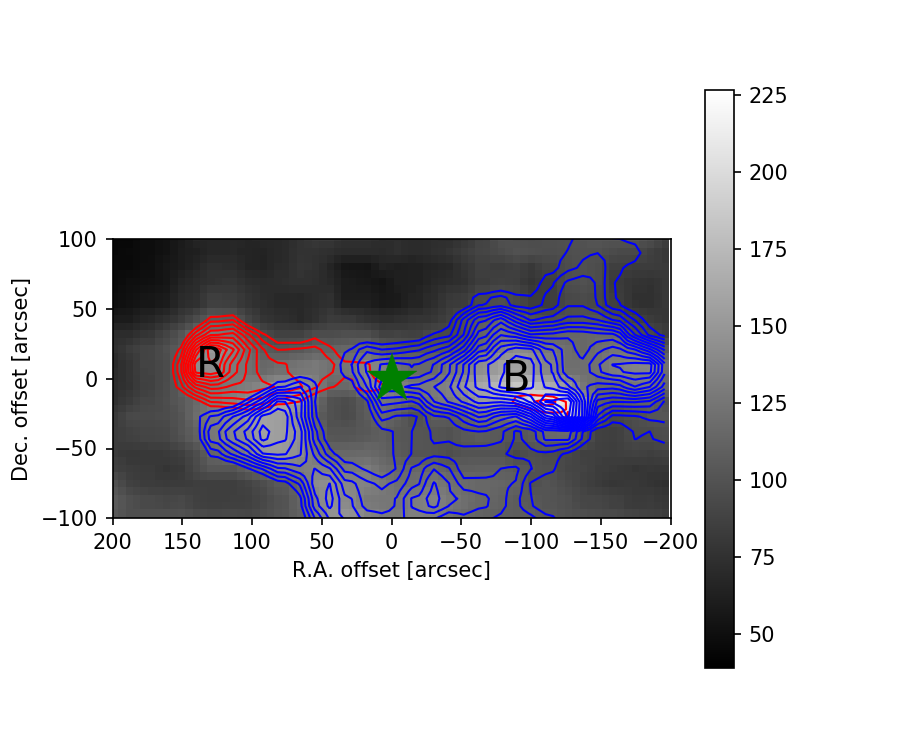
\includegraphics[width=5cm]{Orion_12CO2-1_MMS9_rbcontour_400_modified.png} &   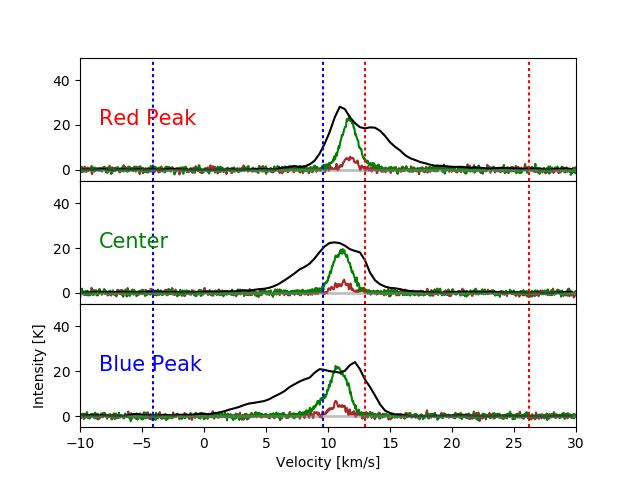
\includegraphics[width=5cm]{Orion_12CO2-1_MMS9_line_profile_400.png} \\
		\end{tabular}
		\label{MMS921}
		\caption{The contour map and the line profile of MMS9. }
	\end{center}
\end{figure}


\noindent\textbf{FIR2} - There is a strong bipolar outflow elongated along the N-S direction as shown in Figure 2. The size is about 30 arcsec, which is smaller than other outflows detected. Red and blue contour intervals are $10\sigma$ starting from $60\sigma$, and $10\sigma$ starting from $100\sigma$, respectively.\\
\textbf{FIR3} - A strong bipolar outflow can be seen along NE-SW direction, with red and blue lobes overlapped with each other as shown in Figure 3. This tells us that the outflow axis is almost parallel to the line of sight. Red and blue contour intervals are $20\sigma$ starting from $40\sigma$, and $20\sigma$ starting from $60\sigma$, respectively. \\
\textbf{FIR6b} - The contour is not so clear because of other IR sources nearby as shown in Figure 4. The outflow is along the NW-SE direction. Red and blue contour intervals are $10\sigma$ starting from $45\sigma$, and $10\sigma$ starting from $110\sigma$, respectively.\\
\textbf{MMS2} - The contour is in a tricky situation, because both red and blue lobes are in the east side of the protostar as shown in Figure 5. The outflow structure on the SW side is the outflow from another prostar, MMS5. It is possible that the outflow structure changed shape because of the turbulence from other protostars. Red and blue contour intervals are $10\sigma$ starting from $30\sigma$, and $10\sigma$ starting from $60\sigma$, respectively.\\
\textbf{MMS5} - There is an outflow structure along the E-W direction as shown in Figure 6. This outflow is much smaller than other bipolar outflows. Red and blue contour intervals are $10\sigma$ starting from $20\sigma$, and $10\sigma$ starting from $40\sigma$, respectively.\\
\textbf{MMS9} = There is a strong outflow along the E-W direction as shown in Figure 7. We can see a smaller red lobe near the center of the blue lobe. Red and blue contour intervals are $10\sigma$ starting from $50\sigma$, and $10\sigma$ starting from $60\sigma$, respectively.\\

\subsubsection{$^{12}$CO J = 1 - 0 Observations}

\begin{figure}[h!]
	\begin{tabular}{ccc}
		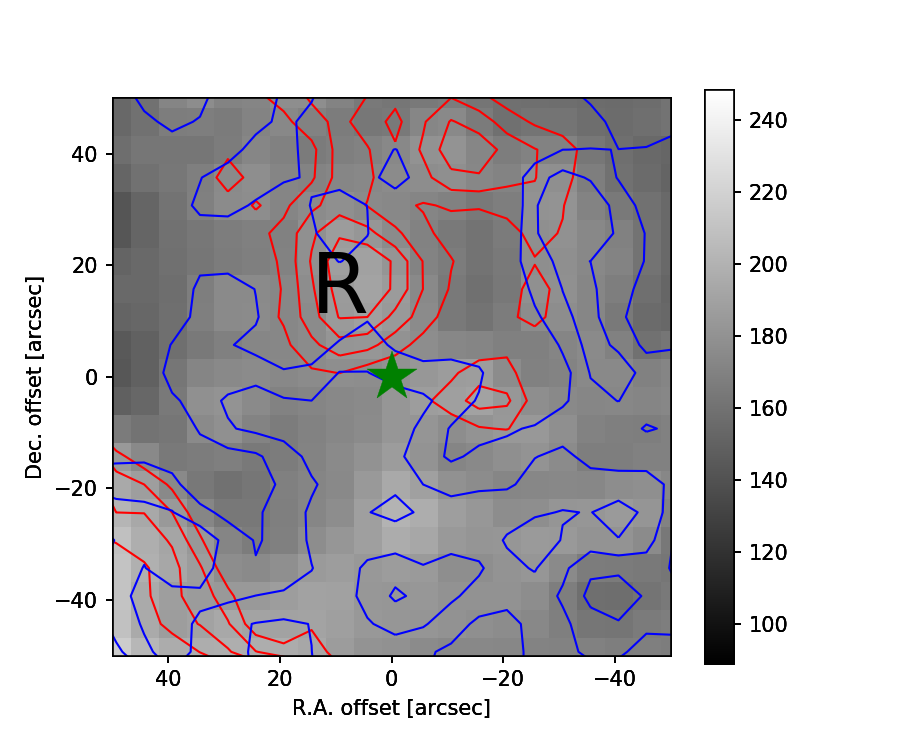
\includegraphics[width = 5cm]{Orion_12CO_NRO_HOPS68_rbcontour_400.png} & 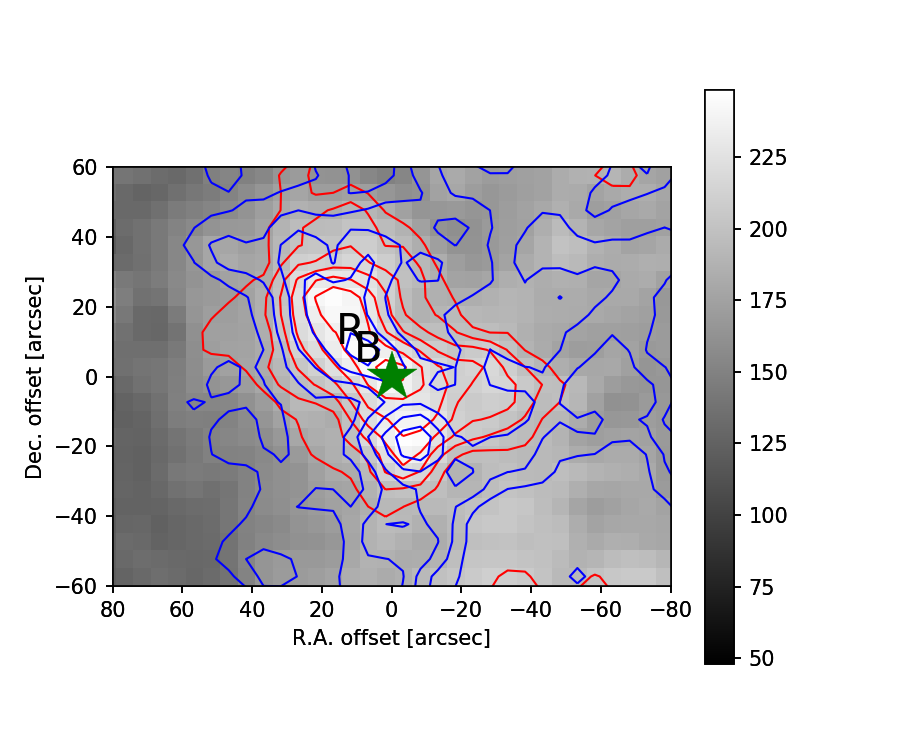
\includegraphics[width = 5cm]{Orion_12CO_NRO_HOPS370_rbcontour_400.png} & 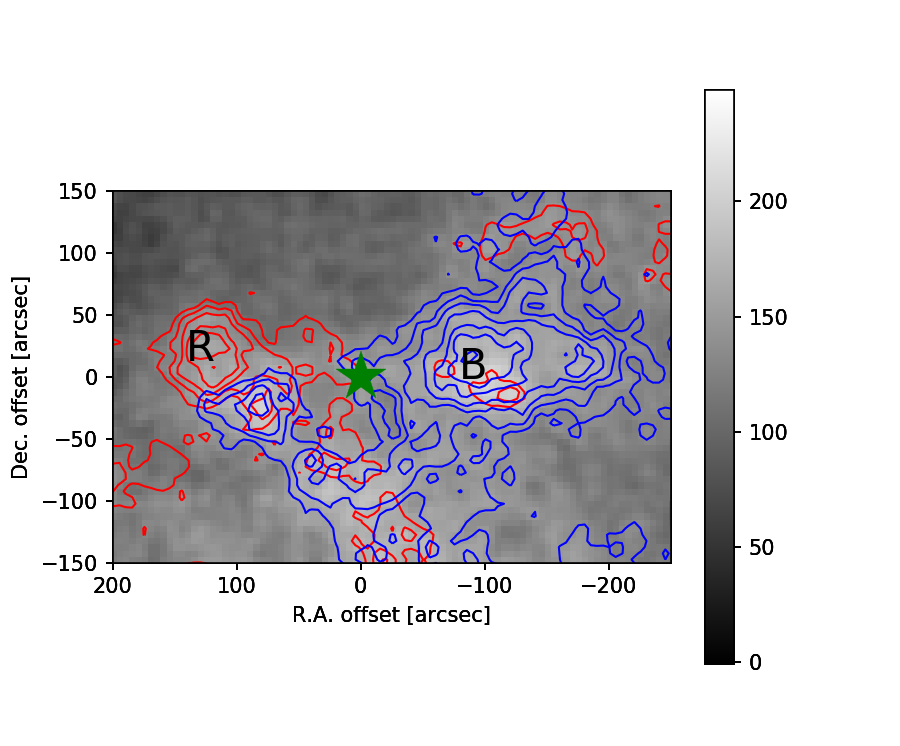
\includegraphics[width = 5cm]{Orion_12CO_NRO_HOPS78_rbcontour_400.png}
		\label{10}
	\end{tabular}
	
	\caption{The contour map of FIR2(left), FIR3(middle), and MMS9(right). }
\end{figure}
 
 
\noindent \textbf{FIR2} - The red lobe is clear on the NW side of the protostar, but the blue lobe is not that clear as shown in Figure 8.\\
\textbf{FIR3} - The outflows are in a similar shape with the J = 2 - 1 observations as shown in Figure 8. The lobe centers are slightly near the protostar.\\
\textbf{MMS9} - The outflows are also in a similar shape with the J = 2 - 1 observations as shown in Figure 8. We can also see that there is a small red lobe near the center of the blue lobe.\\
\newpage

\subsection{Momentum Flux}

The momentum flux within one beam is calculated as the following:

\begin{equation}
\dot{P} = \frac{dP}{dt} = \sum_{v} {\frac{M_B (v) (v/ \cos i)}{D\theta_B / (v \tan i)}}
\end{equation}

$v$ is the velocity offset from $v_{cen}$, $M_B (v)$ is the mass within one beam, $i$ is the inclination within one beam \cite{Hatchell2}.
Then the momentum flux from individual beams are summed in annuli. 

\begin{equation}
F_{\textrm{CO}} = \sum _{annulus} \frac{2\pi \theta_r}{N_{pix}\theta_B}\dot{P}	
\end{equation}

$N_{pix}$ is the number of pixels in a annulus. $\theta_r$ is the distance between each pixel and the outflow center. $\theta_B$ is the beam size \cite{Hatchell2, Marel}.


\begin{table}[h]
	\begin{center}
		\begin{tabular}{c|c|c|c||c|c|c}
			\toprule
			\multirow{3}{1cm}{\textbf{Name}} & \multicolumn{3}{c}{J = 2 - 1} & \multicolumn{3}{c}{J = 1 - 0} \\
			& $\mathbf{F_{R}}$ & $\mathbf{F_{B}}$ & $\mathbf{F_{\textrm{CO}}}$ & $\mathbf{F_{R}}$ & $\mathbf{F_{B}}$ & $\mathbf{F_{\textrm{CO}}}$\\
			& \multicolumn{6}{c}{($M_{\odot} \textrm{km s}^{-1} \textrm{yr}^{-1}$)}\\
			\midrule
			FIR2 & 1.14E-05 & 3.28E-05 & 4.42E-05 & 4.78E-06 & - & 4.78E-06\\
			FIR3 & 4.77E-04 & 7.43E-04 & 1.22E-03 & 1.86E-04 & 3.02E-04 & 4.88E-04\\
			FIR6b & 1.13E-05 & 1.18E-05 & 2.31E-05 & - & - & -\\
			MMS2 & 1.14E-05 & 4.50E-05 & 5.64E-05 & - & - & -\\
			MMS5 & 5.80E-06 & 1.55E-05 & 2.13E-05 & - & - & -\\
			MMS9 & 3.67E-06 & 1.09E-05 & 1.46E-05 & 1.45E-06 & 6.02E-06 & 7.47E-06\\
		\end{tabular}
	\end{center}
	\caption{CO outflow parameters} \label{result}
\end{table}


Table \noindent\ref{result} shows the parameters of the outflows detected. $F_R$ and $F_B$ stands for the outflow forces for the red lobe and the blue lobe respectively. $F_{\textrm{CO}}$ is calculated by adding the two forces, which shows the momentum flux of the protostar. We can see that more outflows were detected by using J = 2 - 1 data, and the momentum flux is 2-3 times higher.\\

\clearpage
\newpage
\subsection{Momentum flux vs. Bolometric luminosity}


\begin{figure}[h!]
	\centering
	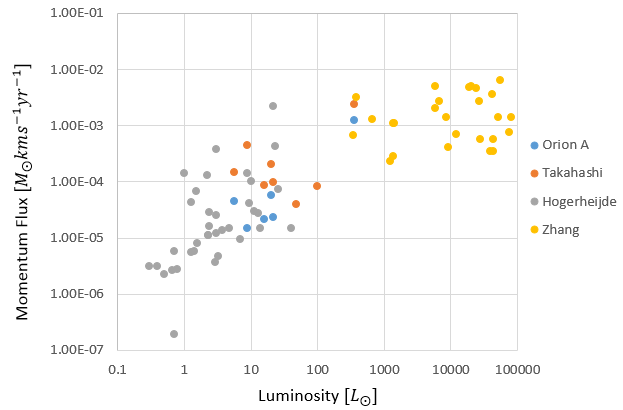
\includegraphics[width=\textwidth]{Luminosity.PNG}
	\caption{Momentum flux difference by emission line energy}
\end{figure}


The graph above shows the relation between the bolometric luminosity and the momentum flux of the outflows from previous studies \cite{Takahashi, Marel, Hogerheijde, Nakamura, Aso, Zhang}. \\ Since the momentum flux of the same protostar is known to vary somewhat depending on the calculation methods\cite{Marel}, the relation between the bolometric luminosity and the momentum flux is difficult to express with the excat formula and only the degree of tendency can be analyzed.
The bolometric luminosity was observed by the Spitzer and Herschel telescopes. Orion A Cloud is a region where stars with medium mass are formed. The fact that the momentum flux of the outflow is proortional to the bolometric luminosity could be checked.

\newpage

\subsection{Momentum flux by emission line energy level}

\begin{figure}[h!]
	\centering
	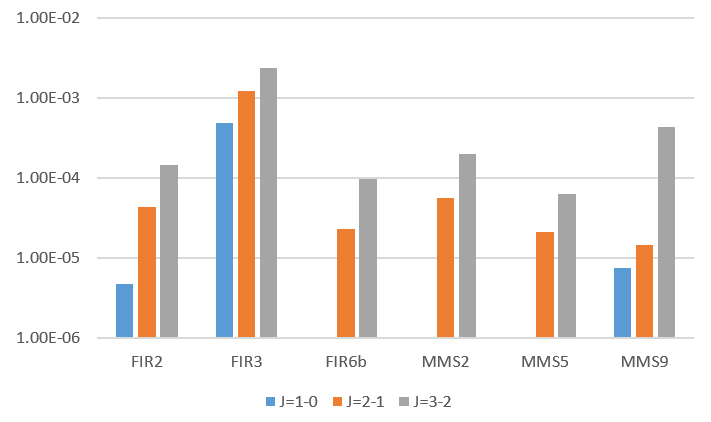
\includegraphics[width=\textwidth]{J.PNG}
	\caption{Momentum flux difference by emission line energy}
\end{figure}

The table compares momentum flux calculated by three different emission lines of the same protostar. The $^{12}$CO J = 3 - 2 observation was made by Takahashi et al \cite{Takahashi}. We can see that it is possible to detect more outflows by using a higher energy emission line of $^{12}$CO. Using data with smaller beamwidth also enhances detecting outflows. The reason that higher energy lines can detect more outflows can be explained as the following. The excitation temperature is higher for emission lines with higher energy. Outflows drag out matter from the protostar's envelope, which has higher temperature than its surroundings. Lines with higher energy are emitted, which has an effect that makes column density higher than usual.

%-----------------------------------------------------
% Conclusion
%-----------------------------------------------------
\newpage

\section{Conclusion}
The main results of this study are the following:
\begin{enumerate}
	\item 6 bipolar outflows were detected from the Orion A Cloud. All outflows were detected by J = 2 - 1 data, and 3 outflows were detected by J = 1 - 0 data.\\
	
	\item The well-known correlation between momentum flux and the bolometric luminosity can be checked. \\
	
	\item It is possible to detect more outflows by using a higher energy emission line of $^{12}$CO. Using data with smaller beamwidth also enhances detecting outflows. The reason that higher energy lines can detect more outflows can be explained as the following. The excitation temperature is higher for emission lines with higher energy. Outflows drag out matter from the protostar's envelope, which has higher temperature than its surroundings. Lines with higher energy are emitted, which has an effect that makes column density higher than usual.\\
	
\end{enumerate}


%-----------------------------------------------------
% Appendix  (Appendix가 없는 경우 이 파트 전체를 제거하시오)
%----------------------------------------------------- 
\clearpage  %%% Appendix를 새 페이지에서 시작
\appendix
\renewcommand{\thesection}{\Alph{section}} %%% TOC에 appendix numbering 재설정
\renewcommand{\thesubsection}{\arabic{subsection}}
\renewcommand{\thesubsubsection}{\arabic{subsubsection}}
\titleformat{\section}[hang] {\normalfont\LARGE\bfseries}{\Alph{section}.}{1em}{} %%% Appendix section title의 재설정
\titleformat{\subsection}[hang] {\normalfont\Large\bfseries}{\Alph{section}.\arabic{subsection}.}{1em}{}
\titleformat{\subsubsection}[hang] {\normalfont\bfseries}{\Alph{section}.\arabic{subsection}.\arabic{subsubsection}.}{1em}{}
\renewcommand{\theequation}{\thesection.\arabic{equation}} %%% Appendix equation numbering 의 재설정
\renewcommand{\thefigure}{\thesection-\arabic{figure}} %%% Appendix figure numbering 의 재설정
\renewcommand{\thetable}{\thesection-\arabic{table}} %%% Appendix table numbering 의 재설정
\setcounter{equation}{0} %%% Appendix equation starting number의 초기화
\setcounter{figure}{0} %%% Appendix figure starting number의 초기화
\setcounter{table}{0} %%% Appendix table starting number의 초기화


%-----------------------------------------------------
%   References 
%-----------------------------------------------------
\clearpage
\begin{thebibliography}{99}\begin{onehalfspace}


\bibitem{Bontemps} Bontemps, S., et al. "Evolution of outflow activity around low mass embedded young stellar objects." Disks and Outflows Around Young Stars. Springer Berlin Heidelberg, 1996. 270-275.
\bibitem{Kang} Kang, Seonmi, et al. "Outflow properties of DIGIT embedded sources." 한국천문학회보 38.1 (2013): 51-51.

\bibitem{Spitzer}Megeath, S. T., et al. "The Spitzer Space Telescope survey of the Orion A and B molecular clouds. I. A census of dusty young stellar objects and a study of their mid-infrared variability." The Astronomical Journal 144.6 (2012): 192.

\bibitem{HerschelFurlan} Furlan, E., et al. "The Herschel Orion protostar survey: spectral energy distributions and fits using a grid of protostellar models." The Astrophysical Journal Supplement Series 224.1 (2016): 5.

\bibitem{Oriondistance}Kounkel, Marina, et al. "THE GOULD’S BELT DISTANCES SURVEY (GOBELINS). II. DISTANCES AND STRUCTURE TOWARD THE ORION MOLECULAR CLOUDS." The Astrophysical Journal 834.2 (2017): 142.
\bibitem{Schulz} Schulz, Norbert S. The formation and early evolution of stars: from dust to stars and planets. Springer Science \& Business Media, 2012.

\bibitem{Berne}Berne, Olivier, Nuria Marcelino, and Jose Cernicharo. "IRAM 30 m Large Scale Survey of $^{12}$CO (2-1) and $^{13}$CO (2-1) Emission in the Orion Molecular Cloud." The Astrophysical Journal 795.1 (2014): 1
\bibitem{Takahashi}Takahashi, Satoko, et al. "Millimeter-and Submillimeter-Wave Observations of the OMC-2/3 Region. III. An Extensive Survey for Molecular Outflows." The Astrophysical Journal 688.1 (2008): 344.
\bibitem{Hatchell2} Hatchell, Jennifer, et al. "Star formation in Perseus-II. SEDs, classification, and lifetimes." Astronomy \& Astrophysics 468.3 (2007): 1009-1024.
\bibitem{Marel} van der Marel, Nienke, et al. "Outflow forces of low-mass embedded objects in Ophiuchus: a quantitative comparison of analysis methods." Astronomy \& Astrophysics 556 (2013): A76.
\bibitem{Hogerheijde}Hogerheijde, Michiel R., et al. "Envelope structure on 700 AU scales and the molecular outflows of low-mass young stellar objects." The Astrophysical Journal 502.1 (1998): 315.
\bibitem{Nakamura} Nakamura, Fumitaka, et al. "Evidence For Cloud-Cloud Collision and Parsec-Scale Stellar Feedback Within the L1641-N Region." The Astrophysical Journal 746.1 (2012): 25.

\bibitem{Aso}Aso, Yoshiyuki, et al. "Dense cores and molecular outflows in the OMC-2/3 region." The Astrophysical Journal Supplement Series 131.2 (2000): 465.



\bibitem{Zhang}Zhang, Qizhou, et al. "Search for CO outflows toward a sample of 69 high-mass protostellar candidates. II. Outflow properties." The Astrophysical Journal 625.2 (2005): 864.

\end{onehalfspace}\end{thebibliography}


%-----------------------------------------------------
%   감사의 글
%-----------------------------------------------------
%\begin{acknowledgements}
%\addcontentsline{toc}{section}{감사의 글}  %%% TOC에 표시
%정말 감사합니다.
%\end{acknowledgements}

%-----------------------------------------------------
%   연구활동 
%-----------------------------------------------------
%\begin{researches}
%\addcontentsline{toc}{section}{연구활동}  %%% TOC에 표시
%\begin{itemize}

%\end{itemize}
%\end{researches}


\end{document} 
